\chapter{Resultados e discussões}
    \label{chp:Resultados}
    
    Antes de coletar os resultado, primeiramente o OpenServer foi compilado e executado no \ac{LPC} conectado à controladora do robô, o qual ficou aguardando conexão via rede \ac{TCPIP}, como esperado.
    
    Já o \textit{OpenClientExemple} foi compilado e executado em dois dispositivos diferentes, um \ac{PC} de arquitetura \textit{x86-64} e um \ac{SBC} de arquitetura \textit{arm64}. Durante a execução do OpenServer a taxa de amostragem foi aferida imprimindo no terminal o tempo que um pacote foi enviado e depois realizando a subtração do tempo atual pelo tempo do último pacote enviado. Os dados foram salvos em uma tabela e convertidos em gráficos.
    
    \section{Teste com PC \textit{x68-64}}
    
        O computador pessoal estava executando o sistema operacional Debian 11 de 64bits, com Kernel Linux Genérico e ambiente de desktop LXDE. É importante ressaltar o ambiente de desktop pois ele pode ser um dos principais responsáveis pelo consumo de processamento do computador, influenciando diretamente nos resultados dos testes. Por este motivo foi escolhido o LXDE, que é um dos ambientes de desktop com menos consumo de processamento que existe.
        
        As informações de hardware mais possivelmente impactantes nos resultados coletados estão listadas abaixo.
        \begin{enumerate}
            \item CPU: Intel Core i7 8550U
            \item GPU: Intel UHD Graphics 620
            \item Memória RAM: DDR4 - 16GB - Single Channel - 2400MHz
            \item Memória ROM: SSD NVME - 512GB - 1500MB/s
            \item Porta ethernet: Gigabit
        \end{enumerate}
        
        Apesar da porta de ethernet ser gigabit, o roteador utilizado só tinha capacidade para conexões de 100 megabits.
        
        Os resultados dos testes de taxa de amostragem do \ac{PC} podem ser vistos na Figura~\ref{fig:resultado_notebook}, onde o eixo horizontal representa cada amostra coletada e o eixo vertical o tempo em microssegundos.
        
        \begin{figure}[h]
            \centering
            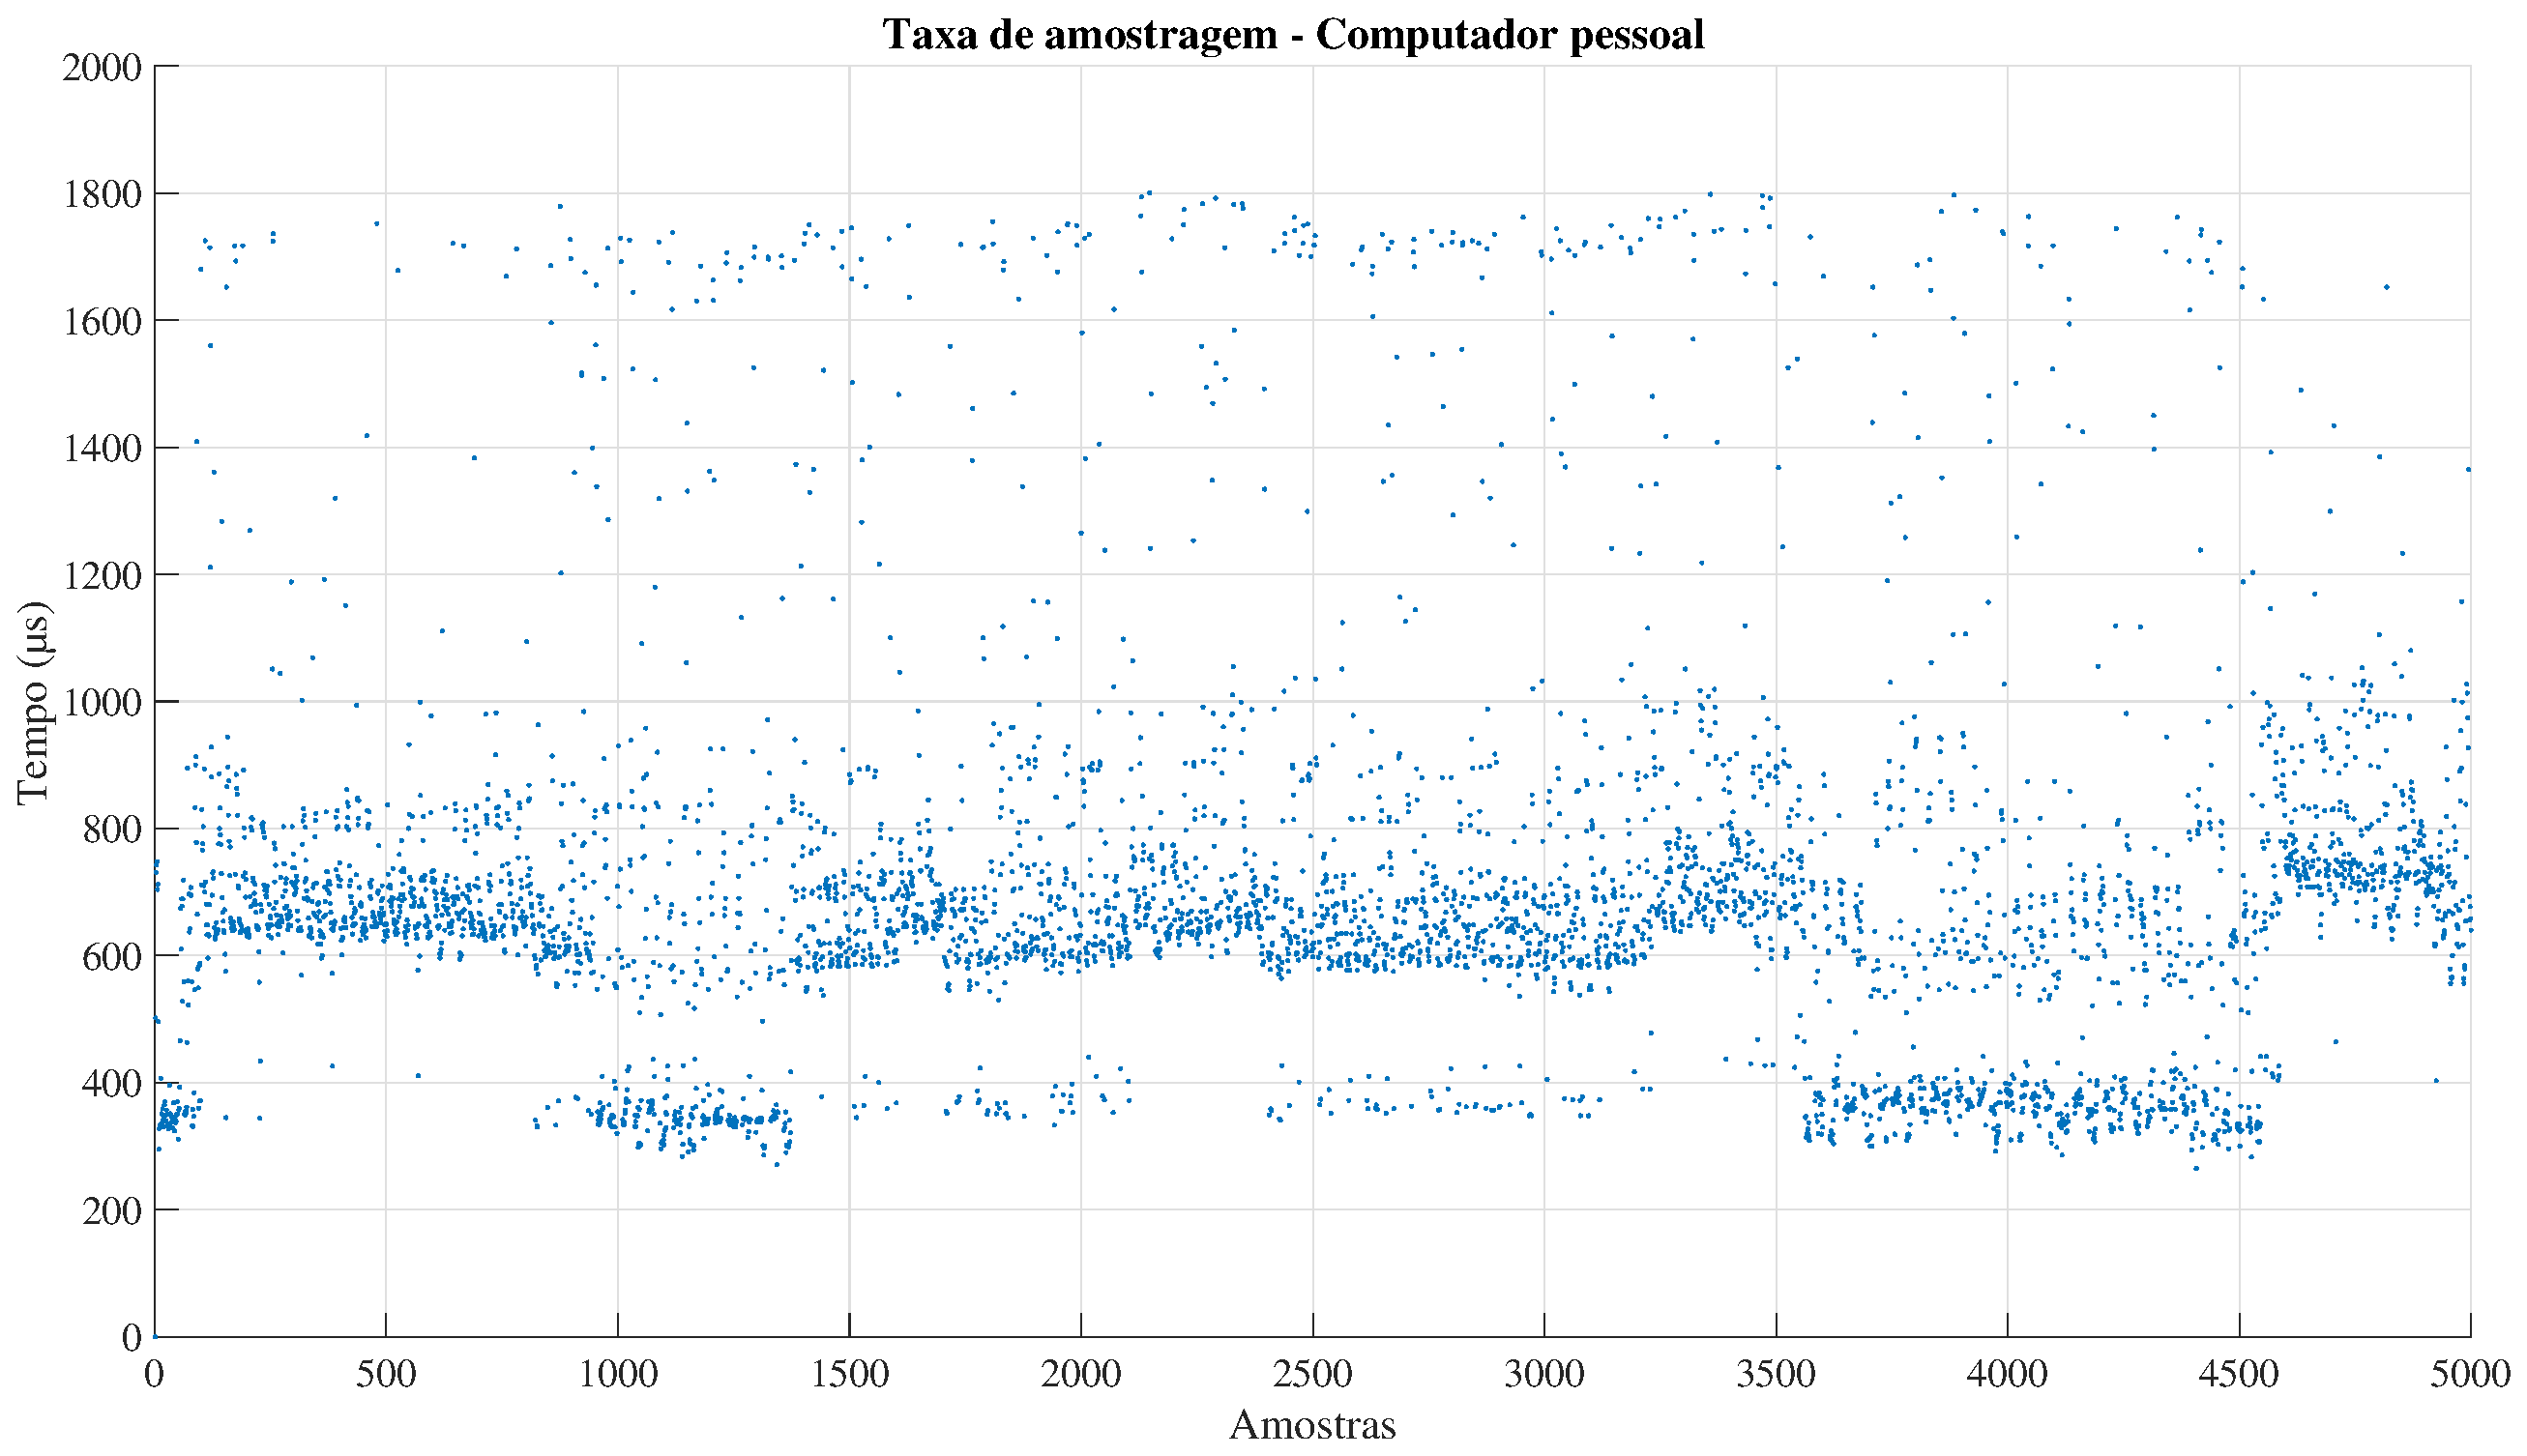
\includegraphics[width=\columnwidth]{imagens/Resultados/testeNote.eps}
            \small 
            \centering 
            \caption{Resultado Notebook}
            \label{fig:resultado_notebook}
        \end{figure}
    
    %single board computer
    \section{Teste com SBC \textit{arm64}}
        
        O \ac{SBC} utilizado nos testes foi o Raspberry Pi 4 Model B executando o sistema operacional Raspberry Pi OS Buster de 64 bits, que na verdade é o sistema operacional Debian 10 com algumas modificações desenvolvidas pela empresa Raspberry. O ambiente desktop é o LXDE-Pi, uma variante do LXDE desenvolvida para o sistema Raspberry Pi OS.
        
        As informações de hardware mais possivelmente impactantes nos resultados coletados estão listadas abaixo.
        \begin{enumerate}
            \item CPU: ARM Cortex A72 QuadCore - 1.5GHz
            \item GPU: Broadcom VideoCore VI - 500MHz
            \item Memória RAM: LPDDR4 - 8GB - Single Channel - 3200MHz
            \item Memória ROM: Cartão SD - 170MB/s
            \item Porta ethernet: Gigabit
        \end{enumerate}
        
        Apesar da porta de ethernet ser gigabit, foi utilizado o mesmo roteador do teste anterior que apenas tem a capacidade para conexões de 100 megabits.
        
        Os resultados dos testes de taxa de amostragem do \ac{SBC} podem ver vistos na Figura~\ref{fig:resultado_PI}, onde o eixo horizontal representa cada amostra coletada e o eixo vertical o tempo em micro segundos.
        
        \begin{figure}[h]
            \centering
            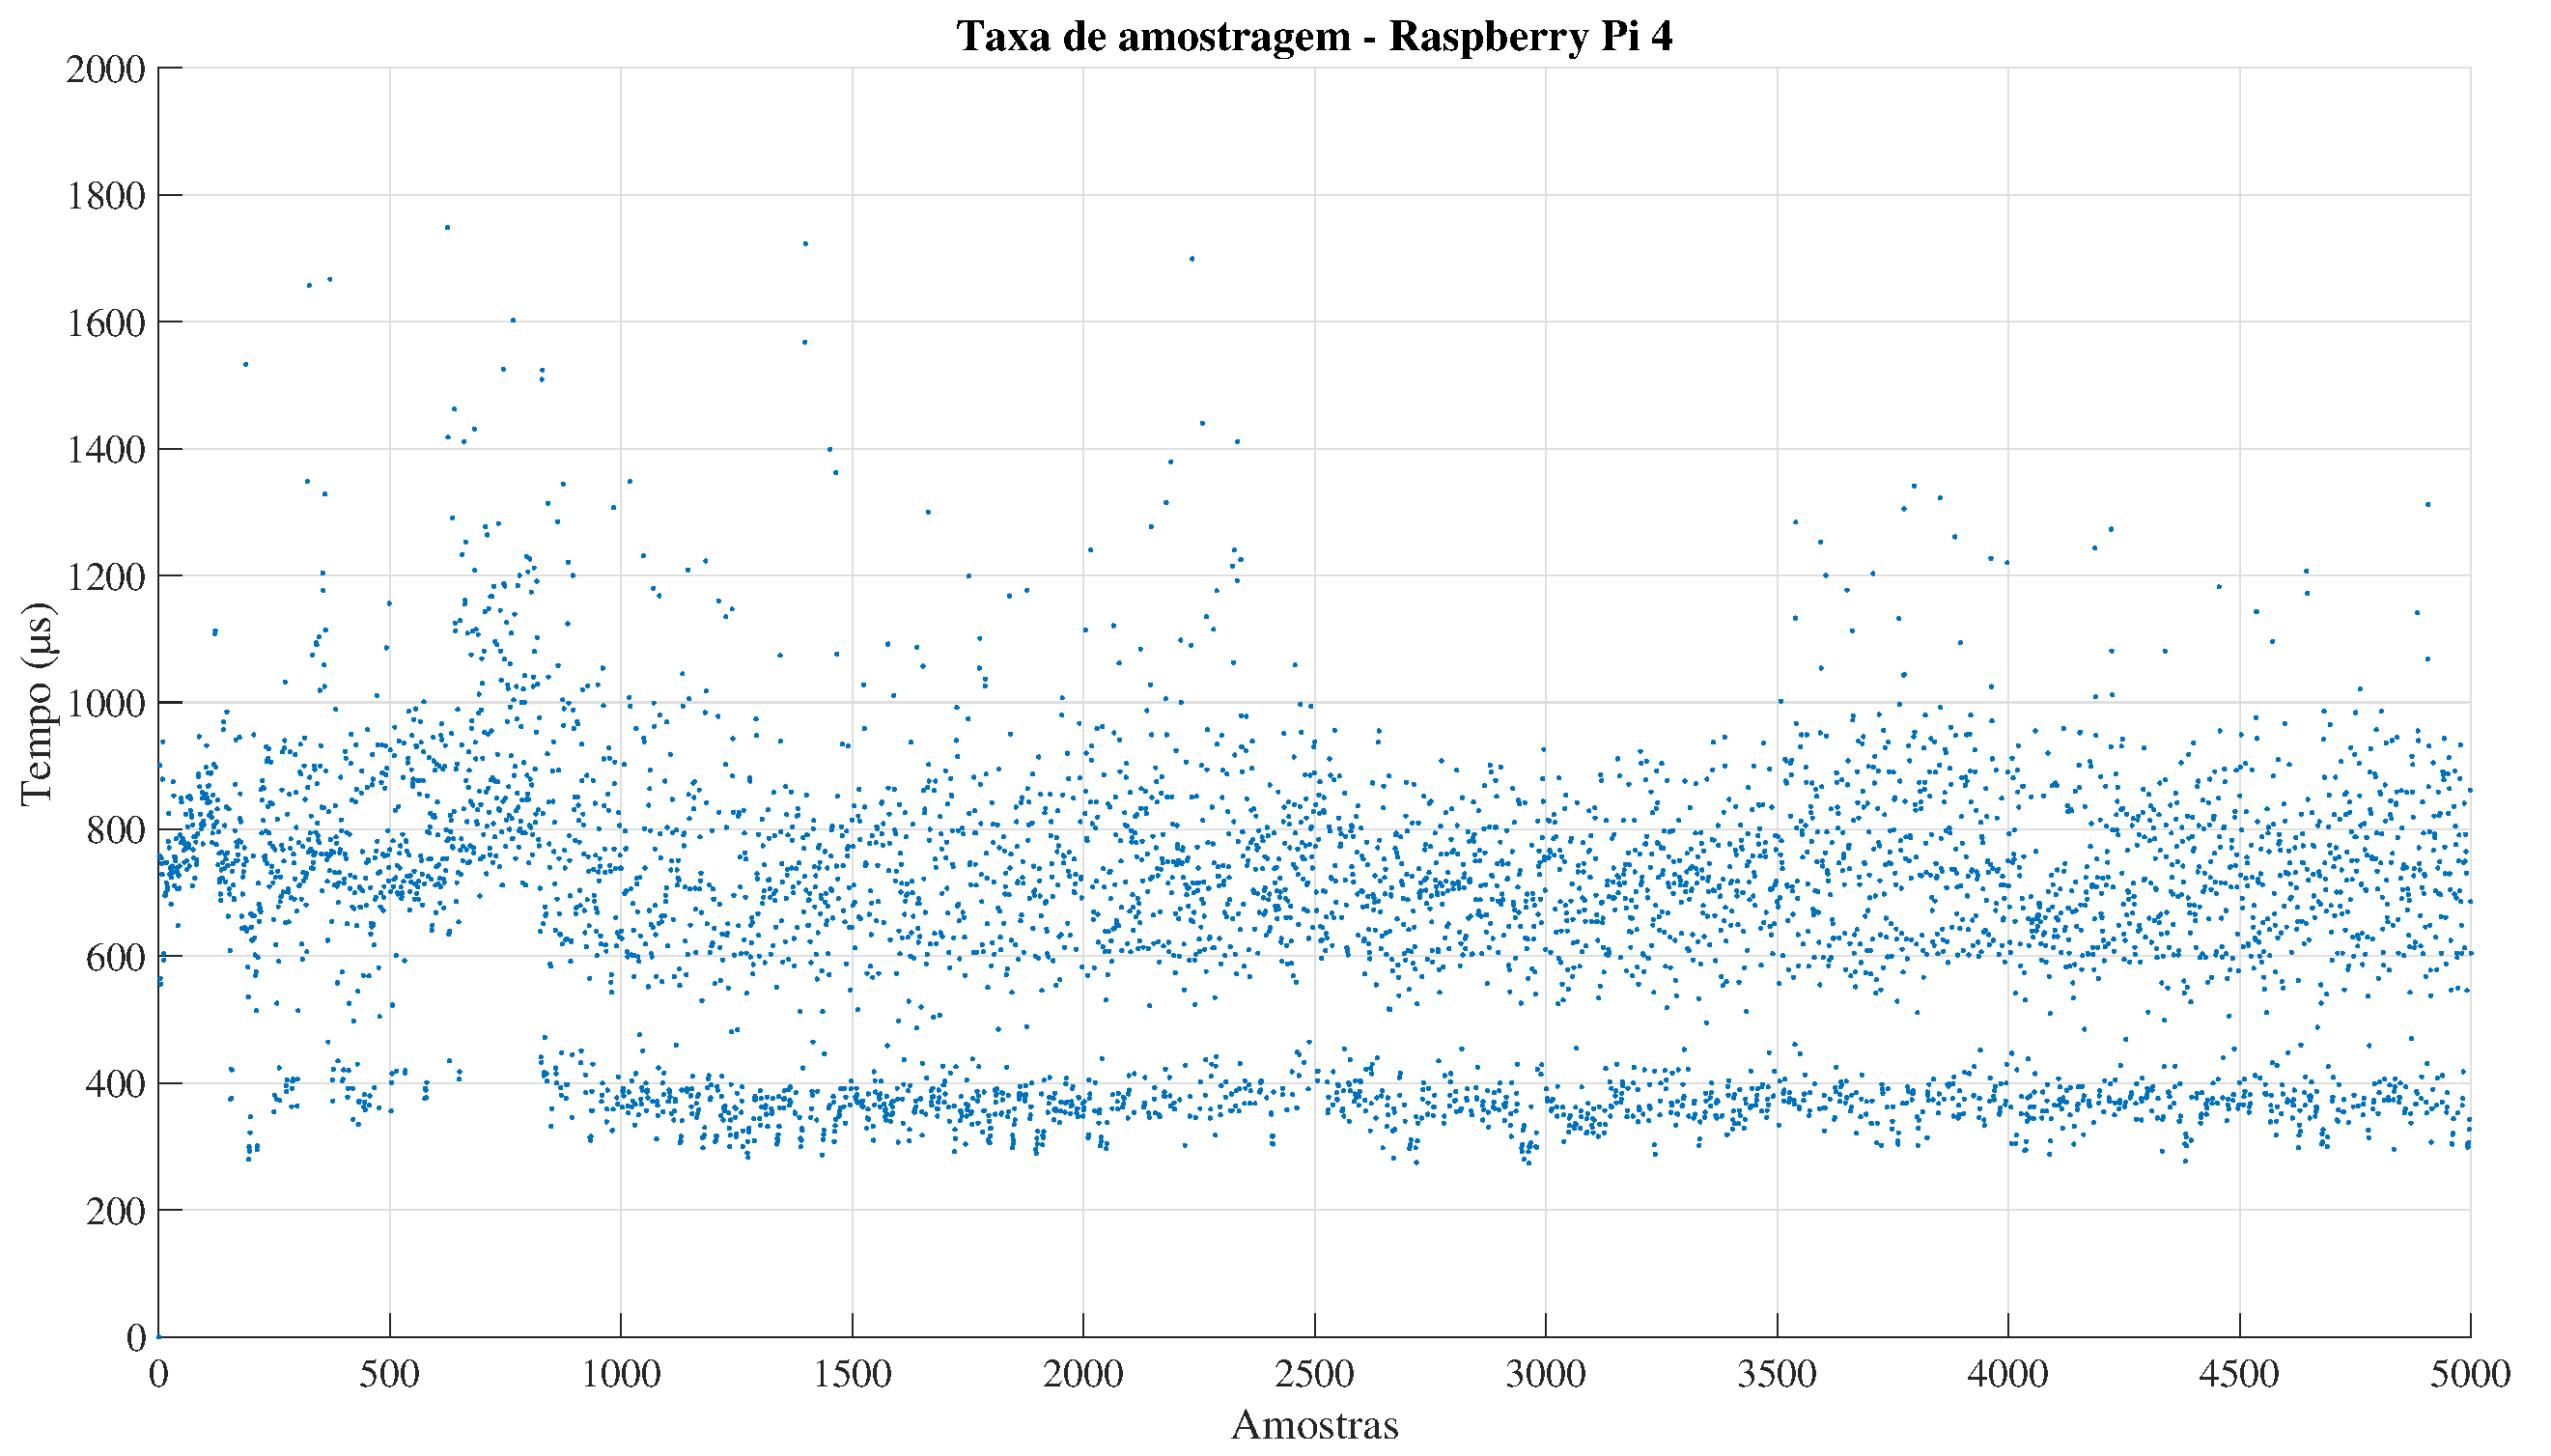
\includegraphics[width=\columnwidth]{imagens/Resultados/testePi.eps}
            \small 
            \centering 
            \caption{Resultado PI}
            \label{fig:resultado_PI}
        \end{figure}
        
    \section{Teste de conexão com outras linguagens, dispositivos e sistemas operacionais}
    
       A fim de verificar se é possível estabelecer a conexão com o OpenServer utilizando outras linguagens de programação e dispositivos foram testadas a linguagem Python e MatLab. A conexão foi estabelecida com sucesso usando a biblioteca padrão \ac{TCPIP} dos mesmos, demonstrando que é possível desenvolver programas clientes em linguagens de programação diferentes da linguagem da biblioteca \ac{eORL}. Como ambos testes foram realizados utilizando o Sistema Operacional \textit{Windows}, foi demonstrando também que podem ser desenvolvidos softwares para outros sistemas operacionais.
       
       Foi testada a comunicação com um dispositivo móvel rodando o sistema operacional \textit{Android} através de um aplicativo genérico de conexão \ac{TCPIP}. O dispositivo móvel estava conectado à rede interna através de conexão sem fio. A comunicação foi bem sucedida, demonstrando que podem ser desenvolvidos softwares clientes para \textit{smartphones} controlarem o braço robótico através do OpenServer e demonstrando também que a rede sem fio pode ser utilizada para conexão com o mesmo.
    
    \section{Discussões}
        
        Em ambos os testes nenhum pacote foi enviado a uma taxa maior que \SI{1800}{\micro\second}, logo é possível estabelecer que \SI{2}{\milli\second} é a menor taxa estável, considerando uma margem de segurança, para os hardwares testados. Apesar de provavelmente essa taxa ser suficiente para atender a maioria das aplicações, acredita-se que ela possa ser melhorada desenvolvendo-se outros protocolos \ac{TCPIP} para transmitir os dados, por exemplo, transmitindo diretamente os valores binários das memórias ao invés de converter em um pacote de strings.
        
        Analisando ambos gráficos, é possível perceber que no computador pessoal ocorreu uma quantidade maior de amostras em torno de \SI{1800}{\micro\second}, logo é possível afirmar que a taxa de amostragem do Raspberry Pi 4 foi mais estável. Provavelmente esse fato se dá que a frequência da memória RAM do Raspberry Pi 4 utilizado é superior, cerca de $30\%$ a mais.
        
        O \textit{OpenClientExemple} foi um programa desenvolvido com o objetivo de testar o interpretador de comandos OpenServer e poder movimentar o robô através do mesmo, logo ele possui uma interface gráfica onde o usuário pode alterar as referências de cada junta, assim testando se o OpenServer está interpretando corretamente as referências enviadas pelo protocolo. Em uma thread separada, os dados da interface gráfica são enviados pelo protocolo TCP/IP e o tempo de envio é imprimido no terminal. Talvez essa abordagem não tenha sido favorável a coletar resultados de taxa de amostragem pois a interface gráfica pode estar consumindo processamento e aumentando a taxa de amostragem, ou talvez a biblioteca de tempo utilizada para executar a thread não seja tão precisa quanto necessário para estes teste.
        
        Para realização de testes mais precisos seria necessário alterar a código do exemplo a fim de retirar a interface gráfica e enviar em loop os pacotes via \ac{TCPIP} pela thread principal, assim dispensando a biblioteca que executa a thread com base no relógio do sistema.
        
        Com base nisso é possível afirmar que a taxa máxima tem que ser analisada para cada dispositivo que vai ser executado o programa cliente e que o OpenServer cumpriu o seu papel de permitir realizar uma taxa de comunicação diferente da controladora e inclusive em taxas não constantes.